\providecommand{\main}{..}
\documentclass[\main/main.tex]{subfiles}

\begin{document}
\graphicspath{{img/}{02_theory/img/}}

% \chapterimage{chapter_head_1.pdf}
\chapter{Ultra-Wideband signals}

\section{Definition of Ultra-Wideband system}

With the $f$\textsubscript{c} is the frequency in which the system has the maximum power density and the frequencies $f$\textsubscript{h} and $f$\textsubscript{L} determine the location where the power of spectral density is 10dB less then the $f$\textsubscript{c}. $B$\textsubscript{frac} is defined as 
\begin{equation}
    B\textsubscript{frac}=\frac{B}{f\textsubscript{c}}
\end{equation} where $B$ is the bandwidth of the system.

In term of high and low frequencies, we have: 
\begin{equation}
    B=2(f\textsubscript{H} - f\textsubscript{L})
\end{equation}
and 
\begin{equation}
    f\textsubscript{c} = \frac{f\textsubscript{H} + f\textsubscript{L}}{2}\
\end{equation} 
so 
\begin{equation}
    B\textsubscript{frac} = \frac{2(f\textsubscript{H} - f\textsubscript{L})}{f\textsubscript{H} + f\textsubscript{L}}
\end{equation}

The Federal Communication Commission (FCC) has define UWB systems as those which have an absolute bandwidth larger than 500Mhz and $f$\textsubscript{c} larger than 2.5 GHz, or have a $B$\textsubscript{frac} larger than 0.2 for system with $f$\textsubscript{c} lower than 2.5GHz. 

Other terms associated with ‘ultra-wideband’ include ‘impulse’, ‘short-pulse’, ‘nonsinusoidal’, ‘carrierless’, ‘time domain’, ‘super wideband’, ‘fast frequency chirp’ and ‘mono-pulse’.

Impulse radio communication systems and impulse radars both utilize very short pulses in the transmission that results in an ultra wide-band spectrum. For radio application, this communication method is also classified as a pulse modulation technique because the data modulation is introduced by pulse position modulation (PPM). 

The UWB signal is noiselike which make the interception and and detection quite difficult. Due to the low-power spectral density, UWB signal cause very little interference with existing narrow-band radio systems. Depending in the attitude of national and international regulatory bodies, this would allow license-free operation of radio systems.

One result of the large bandwidth of UWB is that due to the inverse relationship of
time and frequency. Figure \ref{fig:uwb_versus_other_radio_communication_systems} shows the differences between UWB and other radio systems in the frequency band and power spectral density.

\begin{figure}[H]
    \centering
    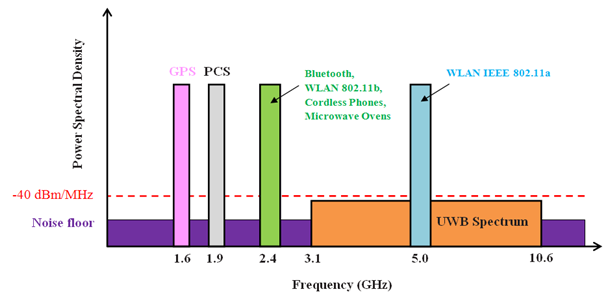
\includegraphics[width=0.8\textwidth]{uwb_versus_other_radio_communication_systems.png}
    \caption{UWB versus other radio communication systems}
    \label{fig:uwb_versus_other_radio_communication_systems}
\end{figure}

\section{Advantages of ultra wide-band}

UWB has a number of advantages that make it attractive for consumer communication applications. In particular, UWB systems:
\begin{itemize}
    \item Have potentially low complexity and low cost
    \item Have noise like signal
    \item Are resistant to severe multipath and jamming
    \item Have good time-domain resolution allowing for localization and tracking application.
\end{itemize}

The low complexity and low cost of UWB systems arises from the essentially base-band nature of the signal transmission. Unlike conventional radio systems, the UWB transmitter produces a very sort time-domain pulse, which is able to propagate without the need of additional RF (radio frequency) mixing stage. The RF mixing stage takes a base-band signal and `inject' carrier frequency or translates the signal to a frequency which has desirable propagation characteristic. The very nature of the UWB signal means it spans frequencies commonly used as carrier frequencies. The signal will propagate well without the need of additional up-conversion and amplification. The reverse process of dow-conversion is also not required in the UWB receiver. Again, this means the omission of a local oscillator in the receiver, and the removal of associated complex delay and phase tracking loop. Consequently, UWB system can be implemented in low cost, low power, integrated circuit process.

Due to the low energy of and the pseudo-random (PR) characteristics of the transmitted signal, the UWB is noiselike, which makes unintended detection quite difficult. Whilst there is some debate in the literature, it appears that low power, noise-like, UWB transmission do not cause significant interference to existing radio systems. The interference phenomenon between impulse radio and existing radio systems is one of the most important topics in current UWB research.

Time-modulation systems offer possibility for high data rates for communication. Hundreds of Mbps have been reported for communication links.

Because of the large bandwidth of the transmitted signal, very high multipath resolution is achieved. The large bandwidth offers huge frequency diversity which, together with the discontinuous transmission, make the UWB signal resistant to severe multipath propagation and jamming/interference. 

The very narrow time domain pulses means that UWB radios are potentially able to offer timming precision much better than GPS and other radio systems. Together with good material penetration properties, UWB signals offer opportunities for short range radar applications such as rescue and anti-crime operations, as well as in surveying and the mining industry. Ine should however understand that UWB does not provide precise target and extreme penetration at the same time, but UWB waveforms present a better choice than do conventional radio systems.

\section{International regulations for UWB signals}

One important feature of a radar and communications transmitter is called the effective isotropic radiated power (EIRP) which can be defined as the product of its gain and input power. Figure \ref{fig:fcc_spectral_mask_for_indoor_uwb_systems} shows the FCC spectral mask of the indoor UWB EIRP emission level. It can be seen that the maximum signal power is limited to -41.3 dBm per MHz throughout the whole UWB frequency range from 3.1 to 10.6 GHz. All the UWB systems and devices must work within this spectral mask for legal operation in order to comply with the FCC standards and regulations.

\begin{figure}[H]
    \centering
    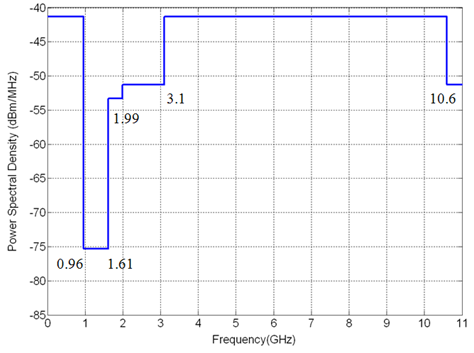
\includegraphics[width=0.7\textwidth]{fcc_spectral_mask_for_indoor_uwb_systems}
    \caption{FCC spectral mask for indoor UWB systems}
    \label{fig:fcc_spectral_mask_for_indoor_uwb_systems}
\end{figure}

\section{Relationship of bandwidth with data rate and power consumption}
As indicated by the Shannon-Harley theorem, there is a direct relationship between capacity and bandwidth and an inverse relationship between bandwidth and power consumption. Their theorem states: 
\begin{equation}
    C=B\log_2(1+\frac{S}{N})
\end{equation} where $C$ is the capacity ($bits/second$), $B$ is the bandwidth, $S$ is the average received signal power over $B$ and $N$ is the average noise over $B$. We observe that for a specific capacity we consume less power with a larger bandwidth. Secondly, because $\frac{S}{N}$ is under a logarithm, it is easier to increase the capacity by increasing of the bandwidth instead of $\frac{S}{N}$. It is common to refer to $\frac{S}{N}$ as SNR, the Signal to Noise Ratio. Figure \ref{fig:capacity_versus_bandwidth_curves_for_uwb_systems_over_awgn_channels} shows the relationship between the bandwidth and the capacity for five different SNRs.

\begin{figure}[H]
    \centering
    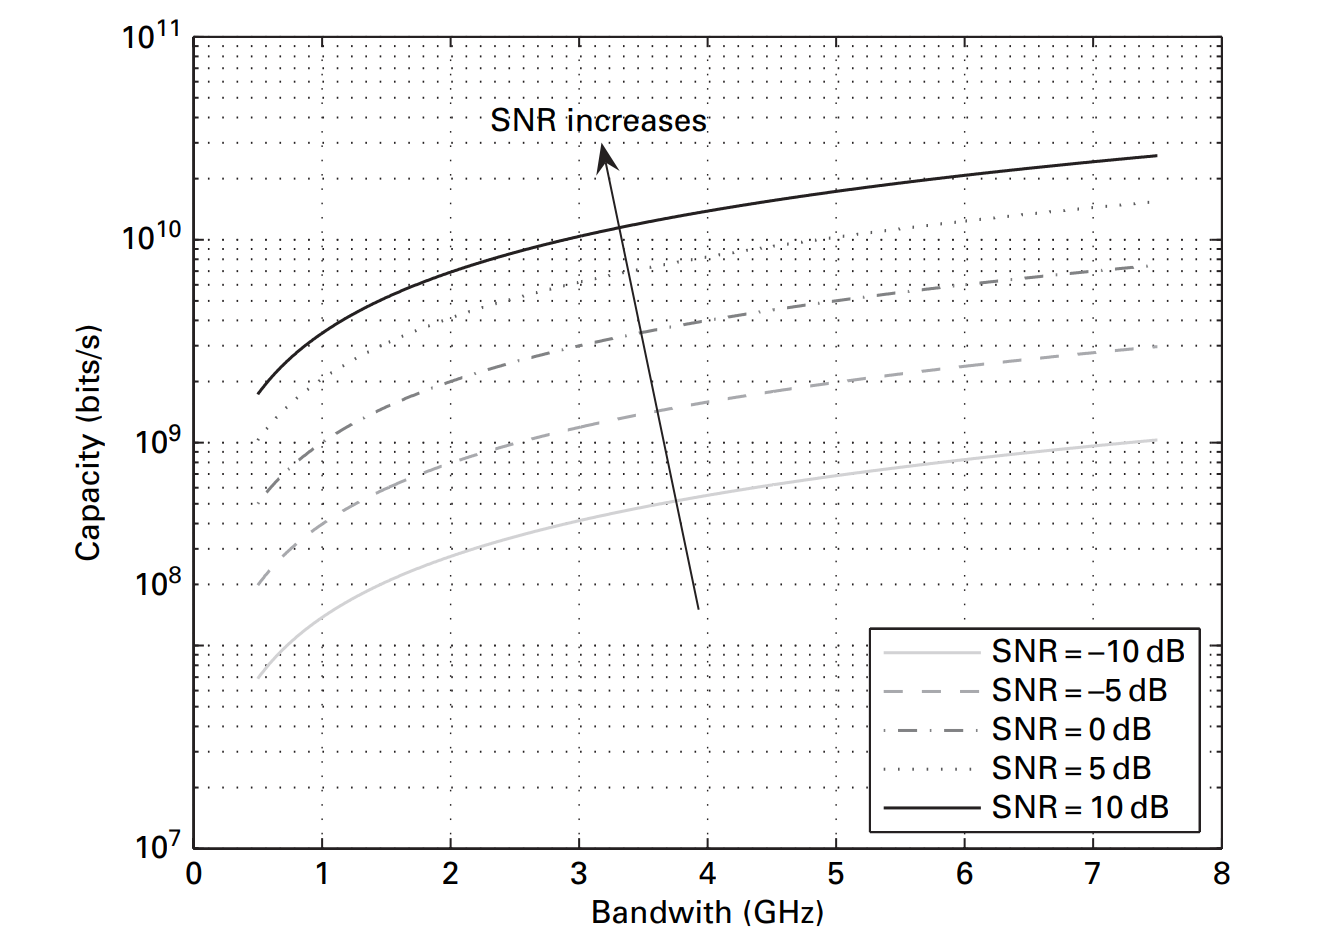
\includegraphics[width=0.8\textwidth]{capacity_versus_bandwidth_curves_for_uwb_systems_over_awgn_channels}
    \caption{Capacity versus bandwidth curves for UWB systems over AWGN channels}
    \label{fig:capacity_versus_bandwidth_curves_for_uwb_systems_over_awgn_channels}
\end{figure}

\section{An UWB modulation scheme: Impulse radio scheme}

Time-modulated ultra wide-band (TM-UWB) communication is based on discontinuous emission of very short Gaussian pulses or other types of pulse waveforms (monocycles), as in figure \ref{fig:an_ir_uwb_signal}. 

In this method, data is transmitted by low duty UWB signals information of the symbol is conveyed by position and/or polarity of the signal. Each symbol correspond to one or more signals. In the following example, two consecutive IR signals represent one symbol. The IR signal can occupy one of the chip-intervals($T\textsubscript{$c$}$) within a frame ($T\textsubscript{$f$}$). A time-hoping (TH) code is used for determining the accurate position of a signal in a dedicated time frame to decrease the chance of interference between UWB systems. 

% In the following example, the TH codes for the symbols are \{2,1\}, \{2,3\} and \{1,0\} respectively, 
% In this example, the information corresponds to the polarity of the signals, so the IR stream represents the binary data `101'. This technique is commonly known as Binary Phase Shifts Keying (BPSK).

\begin{figure}[H]
    \centering
    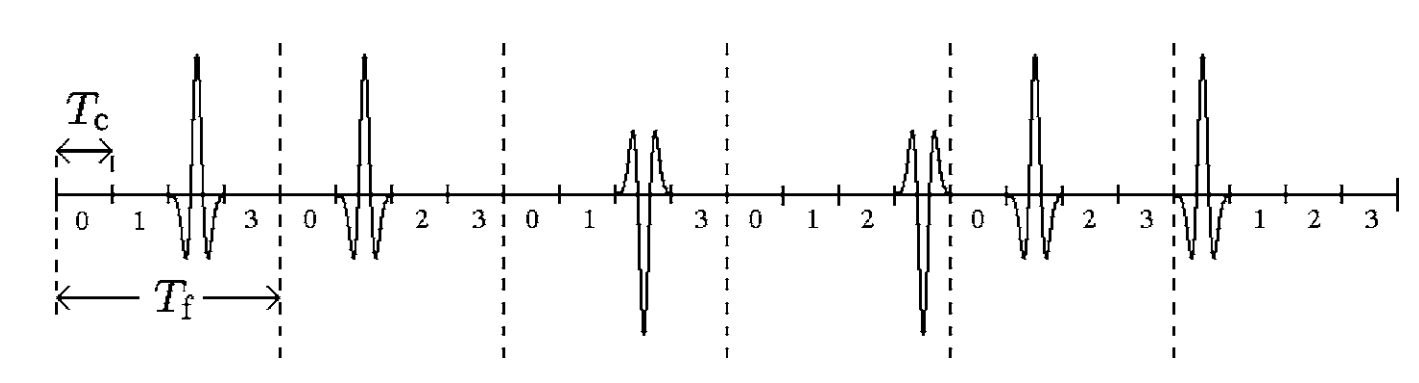
\includegraphics[width=1\textwidth]{an_ir_uwb_signal}
    \caption{An IR UWB signal}
    \label{fig:an_ir_uwb_signal}
\end{figure}

An IR UWB signal, in which two pulses are transmitted per information symbol, and information is conveyed by the polarities of the pulses (BPSK). Hence, +1, -1 and +1 are being transmitted in the example shown in figure \ref{fig:an_ir_uwb_signal}. Note that each pulse resides in an interval of $T\textsubscript{$f$}$ seconds, called a “frame’’, and the positions of the pulses in different frames are determined by a TH (Time-hoping) code, which is {2, 1, 2, 3, 1, 0} in the example, so the first and the second signals are shifted by two and one chip-interval respectively and so on. 

\section{IEEE 802.15.4a standard}
The IEEE established the 802.15.4a study group to define a new physical layer concept for low data rate applications utilizing UWB technology at the air interface \cite{IEEE_Std_802_15_4_2015}. The study group addresses new applications that require only moderate data throughput, but long battery life such as low-rate wireless personal area networks, sensors and small networks.

The IEEE 802.15.4a specifies two optional signaling formats based on IR-UWB and chirp spread spectrum (CSS). The IR-UWB option can use 250–750 MHz, 3.244-4.742 GHz, or 5.944-10.234 GHz bands; whereas the CSS uses the 2.4–2.4835 GHz band. For the IR-UWB there is an optional ranging capability, whereas the CSS signals can only be used for communications purposes. Only the IR-UWB option of the IEEE 802.15.4a standard is studied in this thesis.

\subsubsection{Channel allocations}
As specified above, a UWB device can transmit in one or more of the following bands according to the IEEE 802.15.4 standard:
\begin{itemize}
    \item Sub-GHz: 250 - 750 MHz
    \item Low band: 3.244- 4.742 GHz
    \item High band: 5.944 - 10.234 GHz.
\end{itemize}

Over these three bands, 16 channels are supported for the UWB PHY: one in the sub-GHz band, four in the low band and 11 in the high band. These channels and their center frequencies and bandwidths are listed in table \ref{tab:uwb_channels_for_the_IEEE_802_15_4a_standard}, along with the specification of mandatory channels in each band. Specifically, a UWB device that implements the low band (high band) should support channel 3 (channel 9), whereas the remaining channels in the band are optional.

\begin{table}[H]
    \centering
    \begin{tabular}{ |c|c|c|c|c| } 
        \hline
        Channel No. & Center freq. (MHz) & Bandwidth (MHz) & UWB band & Mandatory \\\hline
        0& 499.2& 499.2& Sub-GHz& Yes \\\hline
        1& 3494.4& 499.2& Low band& No \\\hline
        2& 3993.6& 499.2& Low band& No \\\hline
        3& 4492.8& 499.2& Low band& Yes \\\hline
        4& 3993.6& 1331.2& Low band& No \\\hline
        5& 6489.6& 499.2& High band& No \\\hline
        6& 6988.8& 499.2& High band& No \\\hline
        7& 6489.6& 1081.6& High band& No \\\hline
        8& 7488.0& 499.2& High band& No \\\hline
        9& 7987.2& 499.2& High band& Yes \\\hline
        10& 8486.4& 499.2& High band& No \\\hline
        11& 7987.2& 1331.2& High band& No \\\hline
        12& 8985.6& 499.2& High band& No \\\hline
        13& 9484.8& 499.2& High band& No \\\hline
        14& 9984.0& 499.2& High band& No \\\hline
        15& 9484.8& 1354.97& High band& No \\\hline
    \end{tabular}
    \caption{UWB channels for the IEEE 802.15.4a standard}
    \label{tab:uwb_channels_for_the_IEEE_802_15_4a_standard}
\end{table}

\bib
\end{document}